% Source: Notion page “7. 大小模型协同决策机制”. Generated without rewriting its content.
\chapter{大小模型协同决策机制}

\section{协同架构}

大小模型协同决策模块位于学生模型推理和最终行为结果输出之间，其本质并不是再次进行行为特征提取，而是根据多个模型及数据质量信号决定当前样本应该采用哪一种决策路径。

整体流程可以表示为：

\begin{figure}[htbp]
\centering
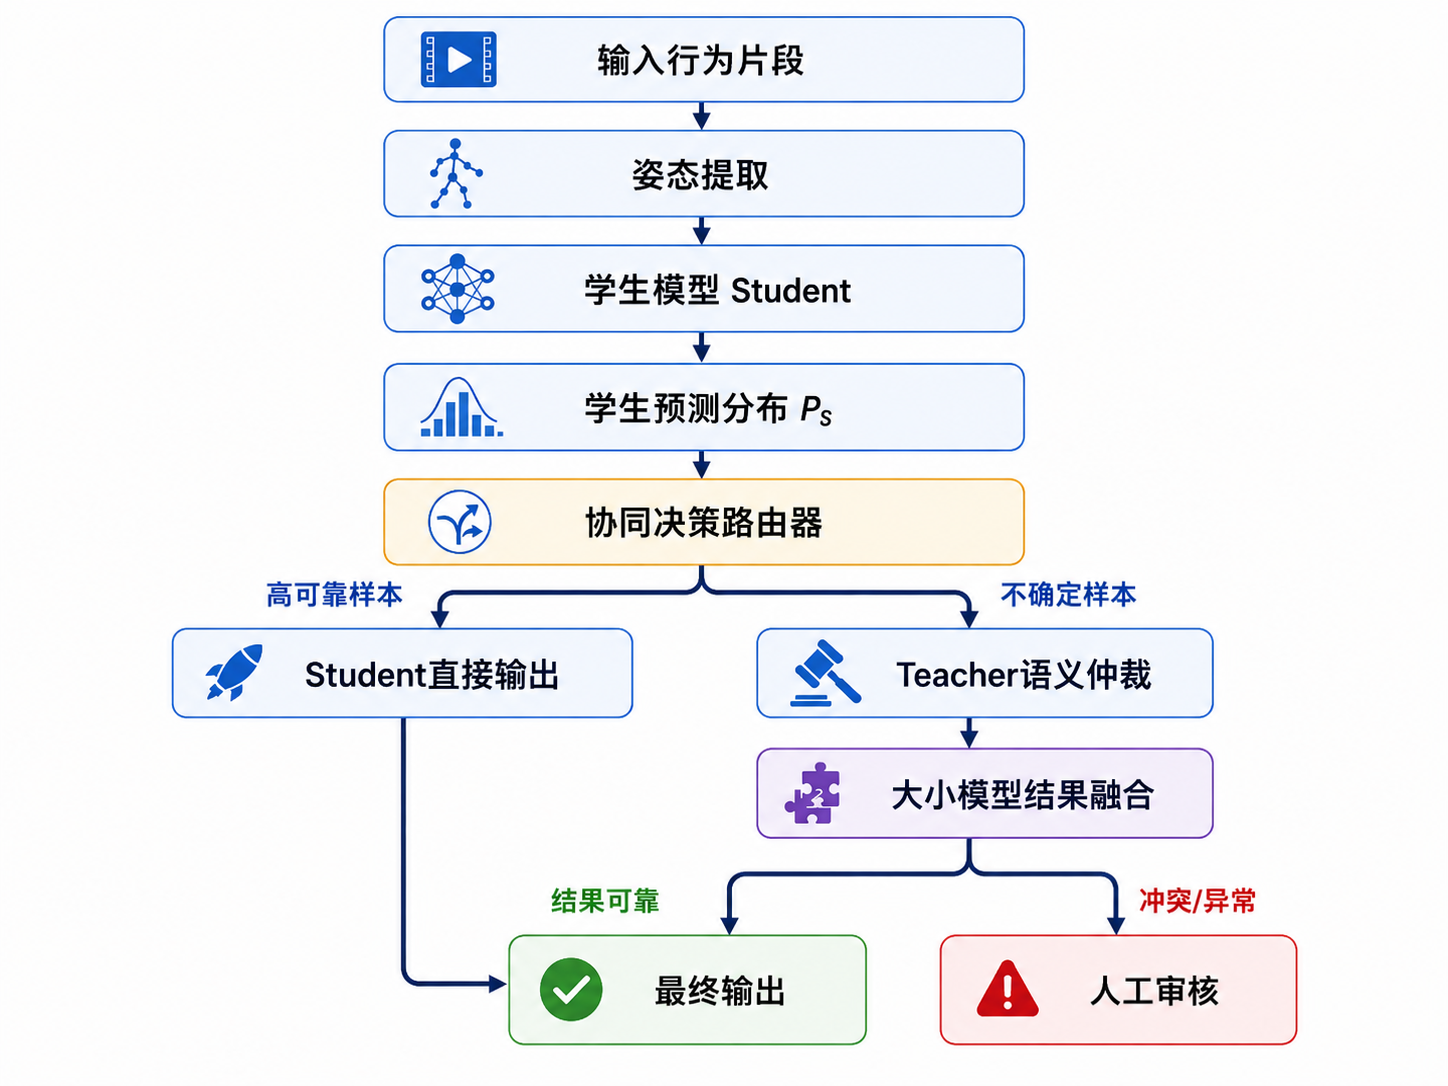
\includegraphics[width=0.96\linewidth,keepaspectratio]{figures/notion_image_04.png}
\end{figure}

\section{大模型触发策略}

为了兼顾识别效果和推理效率，大模型不参与所有样本的识别，而是主要处理学生模型难以稳定判断的样本。系统根据学生模型预测结果和姿态数据质量判断是否需要调用教师模型。

主要考虑以下四类情况。

\subsection{预测置信度较低}

当学生模型最高类别的预测概率较低时，说明模型对当前行为没有形成明确判断。此时直接采用学生模型结果存在较大风险，因此触发教师模型进行进一步分析。

当前系统可将学生模型 Top-1 置信度低于一定阈值作为触发条件，例如：

\[
C_S < 0.70
\]

阈值主要用于识别困难样本，后续可根据验证集表现进一步调整。

\subsection{Top-1 与 Top-2 过于接近}

仅判断最高类别的置信度并不能完全反映模型的不确定性。

例如学生模型输出：

\begin{NotionCode}[plain text]
playful_chase     0.51
conflict_chase    0.47
\end{NotionCode}

虽然最高概率超过 0.5，但两个类别之间差距很小，说明模型实际上难以区分当前行为。

因此系统进一步计算 Top-1 与 Top-2 的概率差：

\[
p_1-p_2
\]

当 Margin 小于设定阈值时，同样调用教师模型。

该机制主要用于发现“嬉戏追逐—冲突追逐”“嬉戏推搡—冲突推搡”等容易发生混淆的样本。

\subsection{姿态数据质量较差}

学生模型依赖人体骨架进行识别，因此关键点缺失、人体遮挡、跟踪错误等问题都会降低预测结果的可信度。

系统根据有效关键点比例和关键点平均置信度计算姿态质量。当姿态质量低于阈值时，即使学生模型给出了较高分类概率，也将其视为需要进一步确认的样本。

此时教师模型可以利用可用的骨架运动信息和结构化语义信息对学生结果进行补充判断。

需要注意的是，姿态质量较差只表示当前学生模型输入不够可靠，并不意味着学生模型结果一定错误。

\subsection{预测结果不稳定}

对于重复推理或历史预测结果，如果同一样本频繁出现 Top-1 类别变化，或者预测置信度波动较大，说明该样本可能位于学生模型的分类边界附近。

系统将此类样本标记为不稳定样本，并调用教师模型进行二次判断。

综合以上条件，只要出现低置信度、Top-1/Top-2 接近、姿态质量较差或预测不稳定中的任意一种情况，即可触发教师模型。这样可以将大模型计算资源集中用于真正困难的样本，而无需对所有视频进行重复推理。


\section{学生模型与教师模型结果融合}

教师模型被触发后，系统同时获得学生模型和教师模型的预测结果。协同决策模块根据两侧结果的一致性和可靠程度形成最终判断，而不是简单规定教师模型直接覆盖学生模型。

当 Student 与 Teacher 预测为同一类别时，说明两种模型基于不同信息来源得到了相同判断，此时系统直接接受该类别作为最终自动识别结果，并保留双方的预测概率和推理信息。

当两个模型预测类别不同，但 Student 本身表现出明显不确定性，例如 Top-1 置信度较低、Top-1 与 Top-2 差距很小，而 Teacher 给出了较为明确的判断时，可以优先采用 Teacher 的结果。

例如：

\begin{NotionCode}[plain text]
Student
playful_push     0.43
conflict_push    0.40

Teacher
playful_push     0.12
conflict_push    0.81
\end{NotionCode}

此时 Student 在两个类别之间存在明显混淆，而 Teacher 对 \(t_p\)ush 的判断更加明确，因此系统采用教师模型结果。

需要注意的是，Teacher 并不具有无条件覆盖 Student 的权限。如果教师模型本身置信度较低、认为证据不足，或者输出存在异常，则不能强制修改学生模型结果。

因此，正常情况下的融合逻辑可以概括为：

\begin{NotionCode}[plain text]
Student 与 Teacher 一致
        ↓
直接确认结果

Student 明显不确定，Teacher 判断明确
        ↓
优先采用 Teacher

双方均较可靠但类别不同
        ↓
进入异常与人工审核流程
\end{NotionCode}

这种方式避免使用复杂的固定权重融合，同时保留了学生模型的运动识别能力和教师模型的语义纠错能力。


\section{冲突、异常与人工审核机制}

当 Student 与 Teacher 无法形成可靠的自动结果，或者系统运行过程中出现模型、输入数据等异常时，当前样本进入异常处理流程。对于仍无法通过自动机制解决的样本，最终进入人工审核队列。

\subsection{模型高置信冲突}

如果 Student 与 Teacher 给出的类别不同，并且双方均具有较高置信度，则认为当前样本存在明显模型冲突。

例如：

\begin{NotionCode}[plain text]
Student：
playful_chase     0.82

Teacher：
conflict_chase    0.79
\end{NotionCode}

这类情况不采用简单概率平均，也不规定某一个模型固定具有更高优先级，而是直接将样本标记为高风险冲突样本。

当前工程可将 Student 与 Teacher 置信度均达到 0.70 以上且类别不同作为高置信冲突条件，该阈值后续可根据实际验证结果调整。

\subsection{教师模型异常}

由于 Teacher 属于生成式模型，其结果在进入协同决策之前需要进行结构化校验，主要检查：

\begin{itemize}
\item 输出类别是否属于六个合法类别；
\item 概率是否处于合法范围；
\item 概率分布是否完整；
\item 最终类别是否与最高概率类别一致；
\item 必要字段是否完整。
\end{itemize}

如果输出不符合要求，可以进行有限次数重新解析或重新推理。若仍然无法得到合法结果，则本次教师结果不参与自动决策。

此外，如果 Teacher 因 GPU 资源不足、模型服务异常、显存不足或推理失败等原因无法运行，而当前样本原本已经因为 Student 不确定而触发 Teacher，则不能重新直接采用原本不可靠的 Student 结果，而应将样本保留到人工审核流程。

\subsection{输入数据异常}

对于视频损坏、无法检测到有效人物、大量关键点缺失或人物跟踪严重失败等情况，系统首先判断剩余信息是否仍然能够支持可靠推理。

如果骨架数据质量较差，则优先结合仍然可靠的关键点、轨迹和结构化语义信息进行判断；当有效信息不足时，不再调用 Teacher 强制分类，而是进入异常或人工审核流程。

如果有效信息已经不足以支持可靠分类，则不强制产生六分类标签，而是将样本标记为异常数据，例如 damaged 或 \(t_o\)f\_scope，避免无效数据产生错误标签。

\subsection{人工审核触发}

当自动协同机制无法安全形成最终结果时，系统将样本送入人工审核队列。主要包括以下情况：

\begin{enumerate}
\item Student 与 Teacher 均具有较高置信度，但预测类别不同；
\item Teacher 明确表示当前证据不足，需要人工确认；
\item 困难样本已经触发 Teacher，但 Teacher 当前不可用；
\item Teacher 多次输出异常，无法获得合法结构化结果；
\item 输入视频或姿态数据严重异常，无法可靠分类；
\item Student 多次推理持续出现类别变化或明显不稳定。
\end{enumerate}

人工审核界面应展示原始视频、骨架结果、Student Top-K 预测、Teacher 预测结果、教师判断依据以及触发审核的具体原因，使审核人员能够结合原始证据完成最终判断。

人工确认后的标签具有最高决策优先级：

\[
y_F=y_H
\]

其中 \(y_H\) 表示人工确认的最终类别。

系统同时保存人工标签、审核原因、备注以及 Student 和 Teacher 的推理快照，保证整个决策过程可追溯。

经过人工确认的困难样本还可以在后续数据筛选后重新加入训练数据，使学生模型逐步学习这些容易产生混淆的决策边界样本，为后续模型迭代提供数据基础。

